\section{Analysis}
\subsection{Complex problems}

% Table moved to experiment.tex for positioning

To further study whether RAP can help stronger LLMs to solve more complex problems, we conduct experiments on the full Blocksworld \cite{valmeekam2023planning} dataset using a more capable LLM, Llama-2 70B \cite{touvron2023llama2}. 

The full \blocksworld \cite{valmeekam2023planning} comprises 602 test cases. We group them based on the minimum number of actions required for each test case. % The distribution of minimum numbers is visualized in Figure~\ref{fig:hist}.
Our experiments are conducted in two distinct settings: \texttt{Easy} and \texttt{Hard}. In \texttt{Easy} setting, we assume prior knowledge of the minimum number of actions for each case. Leveraging this information, we use demonstration cases that share the same minimum number of actions as the test case.
For each group of cases, we randomly select 10 cases to create a pool of demonstration cases, leaving the remaining cases as the test set. During inference, we randomly sample 4-shot demonstration cases from this pool and utilize them to formulate prompts.
% , following a similar format to the examples shown in Appendix~\ref{sec:bw_prompt}.
In the \texttt{Hard} setting, we randomly select 10 cases from the full dataset to form a demonstration pool and subsequently exclude these cases from the test set.
During inference, we randomly sample 4-shot demonstration cases from this global pool, irrespective of the minimum number of actions required for the test case.

We employ chain-of-thought prompting \cite{wei2022chain} as a baseline, and evaluate our RAP$^{(10)}$ (with 10 iterations) with an improved prompting technique (Appendix~\ref{sec:adaptive}). Our experimental results are summarized in Table~\ref{tab:bw_full}. In both the \texttt{Easy} and \texttt{Hard} settings, RAP demonstrates superior performance over CoT by a substantial margin. Notably, when the test case necessitates a larger number of steps (six or more) to solve, CoT exhibits a severe drop in success rates, whereas RAP maintains a relatively high success rate. Comparing these results with Section~\ref{sec:plan}, we additionally conclude that RAP is a general framework able to enhance the reasoning abilities of LLMs, regardless of their intrinsic capabilities.

% \begin{figure}
%     \centering
%     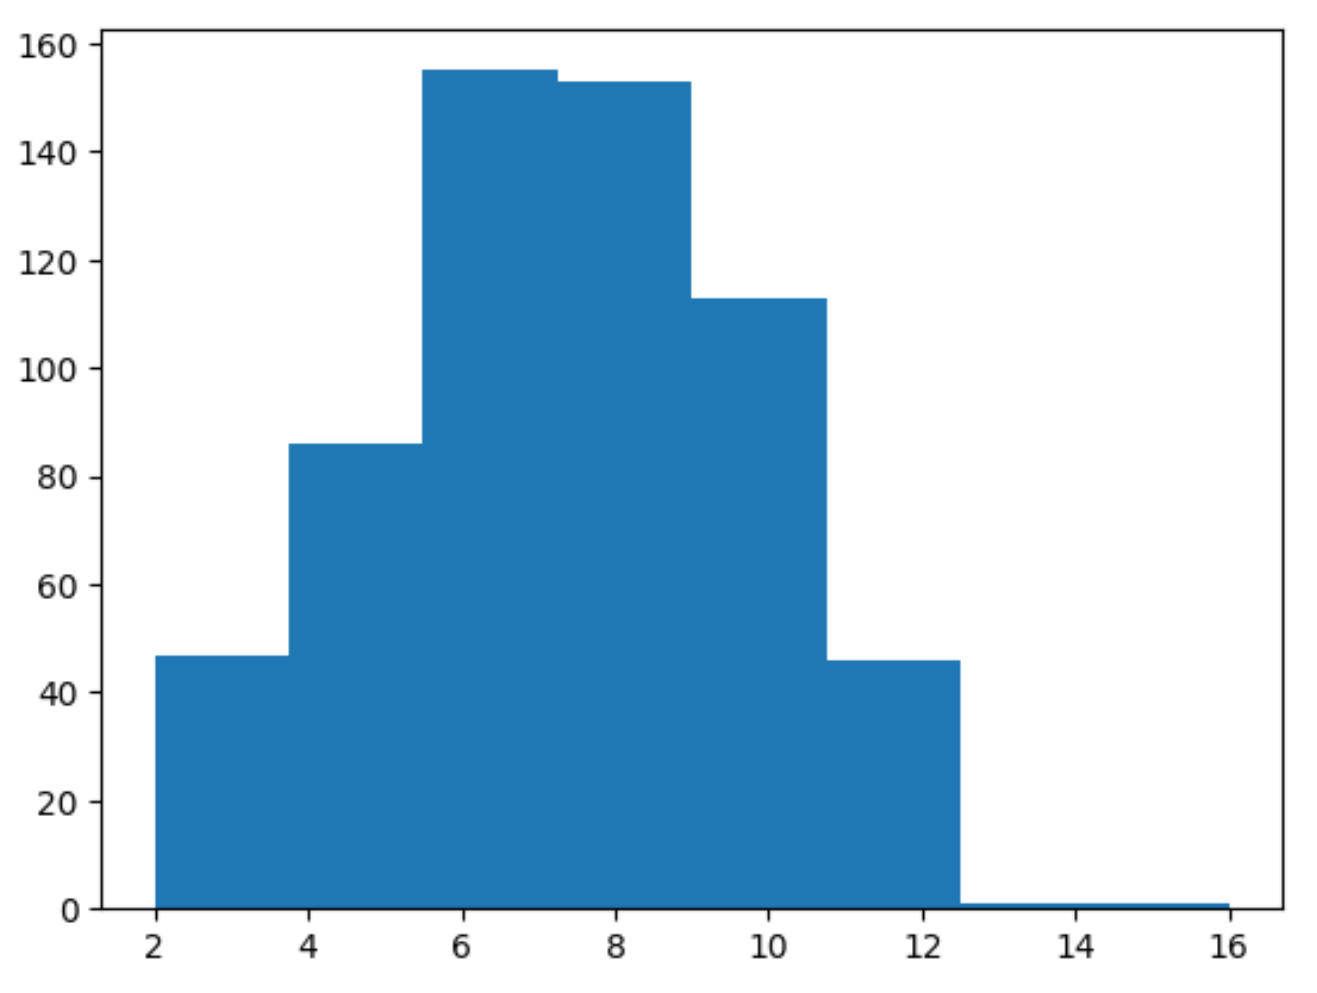
\includegraphics[width=0.9\linewidth]{sections/hist.png}
%     \caption{The statistics of minimal action number for all test cases in \blocksworld}
%     \label{fig:hist}
% \end{figure}


\subsection{Reward Choice}

\label{sec:ablation}
In our main experiments, we choose the combination of rewards in our current experiments based on heuristics and our exploratory experiments. To understand the effects of the reward choice for LLM reasoning, we supplement comprehensive experiments on rewards for plan generation (Table~\ref{tab:bw_ablation}) and math reasoning (Table~\ref{tab:gsm8k_ablation}).

Generally, the combination of multiple rewards contributes to the performance. However, the effects of a reward depends on the nature of tasks. For example, the action likelihood reward is essential for plan generation, but not very helpful to mathmatical reasoning. More discussions are in Appendix~\ref{sec:reward_appendix}.


% \vspace{-5pt}
\section{Conclusion}
% \vspace{-5pt}




In this paper, we present Reasoning via Planning (RAP), a novel LLM reasoning framework that equips LLMs with an ability to reason akin to human-like strategic planning. Our framework, which repurposes the LLM to act as both a world model and a reasoning agent, enables the LLM to simulate states of the world and anticipate action outcomes, and achieve an effective balance between exploration and exploitation via Monte-Carlo Tree Search. Extensive experiments on a variety of challenging reasoning problems demonstrate RAP's superiority over several contemporary CoT-based reasoning approaches, and even the advanced GPT-4 in certain settings. 

% RAP's flexibility in formulating rewards, states, and actions further proves its potential as a general framework for solving diverse reasoning tasks. We posit that RAP, with its innovative melding of planning and reasoning, has the potential to redefine the way we approach LLM reasoning - essentially forging a new pathway toward achieving human-level strategic thinking and planning in artificial intelligence.
